\begin{question}[section=2,name={23.7.2014},mode=exm,type=bsp,tags={20140723}]
Eine fremderregte Gleichstrommaschine hat folgende Daten. Generatorkennlinie ist gegeben (siehe Abb.\ref{fig:20140723})\\
\begin{tabular}{L{2cm}l}
$I_{N}$ \dotfill &$100~A$\\
$U_{A,N}$ \dotfill & $400~V$ \\
$n_N$ \dotfill & $2940~\frac{U}{min}$\\
$n_0$ \dotfill & $3000~\frac{U}{min}$
\end{tabular}
\begin{enumerate}
\item Berechnen Sie den Ankerwiderstand $R_A$ der Gleichstrommaschine und die Spannungskonstante $k_1 \phi_N$ im Nennpunkt der Maschine. (\addpoints{2})
\item Wie groß ist das Nennmoment $M_N$ der Gleichstrommaschine. (\addpoints{1})
\item Die Gleichstrommaschine wird mit konstanter Ankerspannung $U_A = 400V$ versorgt, es liegt \underline{halbe} Nennerregung an. Berechnen Sie die Drehzahl in Abhängigkeit des Moments $n=f(M_i)$ und skizzieren Sie diesen Verlauf im Bereich $\pm M_N/2$. (\addpoints{3})
\item Die Maschine wird nun als \underline{Nebenschlussgenerator} betrieben. Skizzieren Sie das Ersatzschaltbild des Generators. Der Gesamtwiderstand im Erregerkreis ist konstant und beträgt $R_E = 45~\Omega$ (Summe aus Spulen und Vorwiderstand). Aus dem Leerlaufversuch konnte folgende Kennlinie des Erregerflusses ermittelt werden. Ermitteln Sie bei konstanter Drehzahl $n = 3000 ~U/min$ die Ankerspannung $U_A$ sowie den Erregerstrom $I_E$ für den leerlaufenden Generator. (\addpoints{4})
\end{enumerate}
\begin{figure}[H]
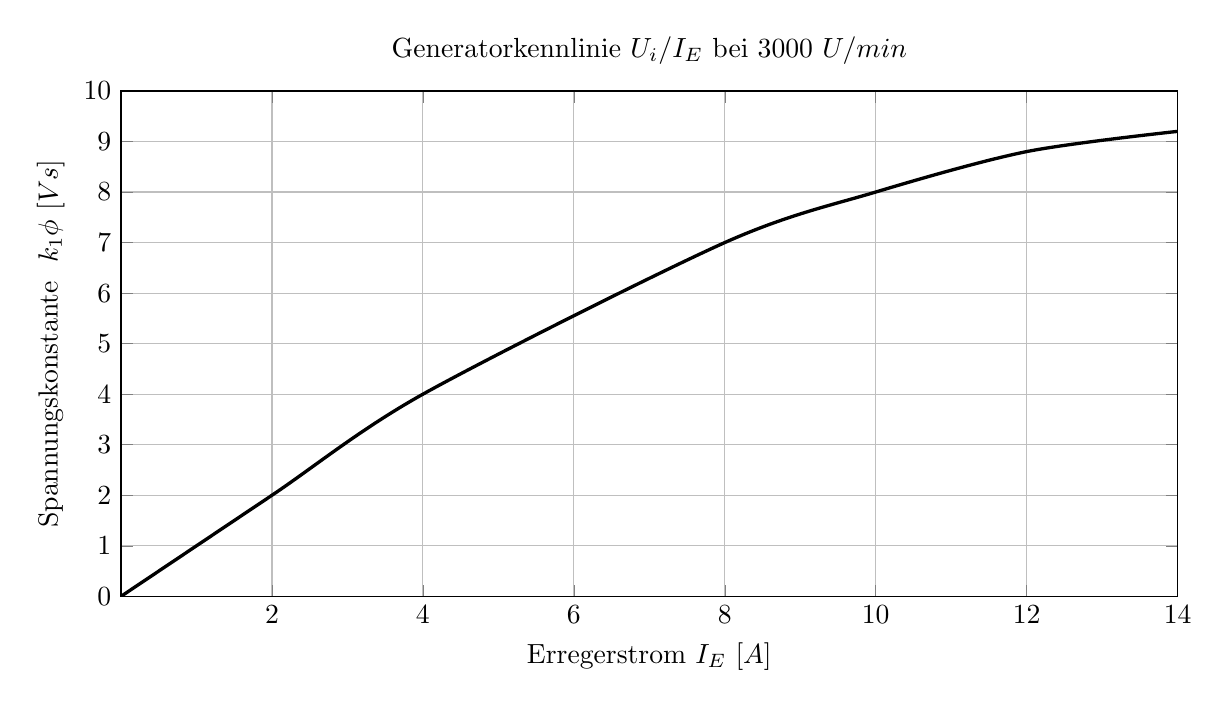
\begin{tikzpicture}
\begin{axis}[title={{Generatorkennlinie} $U_i/I_E$ {bei} $3000 ~U/min$},xlabel={{Erregerstrom }$I_E \, \left[A\right]$ }, ylabel={{Spannungskonstante } $k_1 \phi \, \left [Vs\right]$},
xtick= {2,4,6,8,10,12,14},width=15cm,height=8cm,
xmin = 0,xmax = 14,
ytick= {0,1,...,10},
ymin = 0 , ymax = 10,grid=major]
\addplot+
[id=exp,color=black,mark=none,smooth, very thick] coordinates {
	( 0,0)
	(2,2)
	(4,4)
	(8,7)
	(10,8)
	(12,8.8)
	(14,9.2)
};
\end{axis}
\end{tikzpicture}
\caption{Generatorkennlinie} \label{fig:20140723}
\end{figure}
\end{question}
\begin{solution}
\begin{enumerate}
\item Im Leerlauf ist der Ankerstrom Null und mittels Glg.(\ref{glg:Ankerspannungsgleichung}) lässt sich die Spannungskonstante errechnen.
\begin{align}
U_{A,N} &= \frac{k_1 \cdot \phi}{2 \pi} \cdot \frac{n_0}{60} \cdot 2 \pi\\
k_1 \cdot \phi &= 8~Vs\\
k^{'} \cdot \phi &= \frac{k_1 \cdot \phi}{2 \pi} = 1,273~Vs
\end{align}
Um den Ankerwiderstand berechnen zu können wird die Ankernennspannung benötigt. Diese errechnet sich aus der Spannungskonstante mit der Leerlaufdrehzahl. Anschließend wird mit (\ref{glg:Ankerspannungsgleichung}) der Ankerwiderstand durch umformen errechnet.\\
\begin{align}
U_{A,N} &= \frac{k_1 \Phi}{2 \pi} \cdot \frac{n_0}{60} 2 \pi = 400~V\\
R_A &= \frac{U_{A,N} - \frac{k \Phi}{2 \pi} \cdot \frac{n_N}{60} 2 \pi}{I_A}=80~m \Omega\\
\end{align}
\item Das Moment errechnet sich mit (\ref{glg:Ankermoment}).\\
\begin{equation}
M_N=\frac{k \Phi}{2 \pi} \cdot I_N =127,3~Nm
\end{equation}
\item Das Ankermoment (\ref{glg:Ankermoment}) wird auf $I_A$ umgeformt und in (\ref{glg:Ankerspannungsgleichung}) eingesetzt und auf $\Omega$ umgeformt, wobei die Hälfte der Erregung $k^{'} \Phi$ eingesetzt wird und Anschließend mit $\frac{60}{2 \pi}$ mulitpliziert wird um auf $n$ zu kommen.
\begin{equation}
n(M_i) = \frac{U_A - R_A \frac{2 M_i}{k^{'} \Phi}}{k^{'}\Phi} \cdot 2 \cdot \frac{60}{2 \pi} =6000-0,197 \cdot M_i
\end{equation}
\textbf{TODO:} Programmiere oder zeichne die Grafik und scan sie ein und lade sie hoch!
\item \textbf{TODO:} Programmiere oder zeichne die Grafik für den Nebenschlussgenerator und scan sie ein und lade sie hoch! Da die Spannungskonstante von dem Erregerstrom abhängig ist, kann hier kein konstanter Wert eingesetzt werden. Es wird die Steigung $k^{'} \phi/I_E$ ermittelt, welche dann als Linie in Abb.(\ref{fig:20140723}) eingezeichnet wird. Bei der Berechnung wird von Glg.(\ref{glg:Ankerspannungsgleichung}) ausgegangen und auf $k^{'} \phi/I_E$ umgeformt.
\begin{align}
U_A &= (R_E +R_A)  I_A  + k^{'} \phi \cdot \Omega_m\\
\frac{k_1 \phi}{I_E} &= \frac{R_E +R_A}{\Omega_N}\cdot 2 \pi = 0,901
\end{align}
Eine Gerade mit der Steigung $0,901$ einzeichnen und bei dem Schnittpunkt ablesen. $I_E= 7,4~A$ und $R_E \cdot I_E = 315~V$.
\end{enumerate}
\end{solution}